We will now present a series of definitions and results that let us
understand the premises of the \rulelabel{E-Pull-Wait} rule, examine
the merge operation in closer detail, and appreciate the need for
constraining the branching structure. First, we formalize the
intuitive notation of the ancestor relationship between versions of a
legal branching history (i.e., a branching history generated by the
rules in Fig.~\ref{fig:opsem}):

\begin{definition} [\bfseries Ancestor]
Version $v_1$ is a ancestor of version $v_2$ under a history
$H$ (written $\under{H}{v_1 \preceq v_2}$) if and only if one of the
following is true:
\begin{itemize}
  \item There exists a branch $b$ in $H$ (i.e., $\exists(t\in
  dom(H)).\,H(t) = b$) in which $v_2$ immediately succeeds
  $v_1$,
  \item There exists a branch $b$ in $H$ that contains $(v_2, 
  \C{FORK}\; (v_1,f_1)::b_1)$, for some $f_1$ and $b_1$,
  \item There exists a branch $b$ in $H$ that contains
  $(v_2, \C{MERGE}\;(v_1,f_1)::b_1)$, for some $f_1$ and $b_1$,
  \item $v_1 = v_2$, or $v_1$ is transitively a ancestor of
  $v_2$, i.e., $\exists v.~ \under{H}{v_1 \preceq v} \conj
  \under{H}{v \preceq v}$ 
\end{itemize}
\end{definition}

Ancestor relation is therefore a partial order (reflexive, transitive,
anti-symmetric) with a greatest lower bound (the initial version).
Thus, for any two versions in a legal history, there exist at least
one common ancestor. Ancestor relationships among the common ancestors
let us define the notion of a least common ancestor (LCA):

\begin{definition} [\bfseries Least Common Ancestor]
Version $v$ is said to be a common ancestor of versions $v_1$ and
$v_2$ under a history $H$ if and only if $\under{H}{v \preceq v_1}$
and $\under{H}{v \preceq v_2}$. It is said to be the least common
ancestor (LCA) of $v_1$ and $v_2$, iff there does not exist a $v'$
such that $\under{H}{v' \preceq v_1}$ and $\under{H}{v' \preceq v_2}$
and $\under{H}{v \preceq v'}$.
\end{definition}

\begin{figure}
\centering
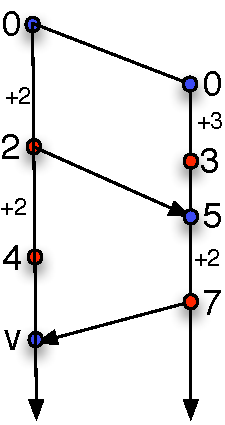
\includegraphics[scale=0.6]{Figures/merge-needs-lca}

\caption{This example of a grow-only counter illustrate why \C{merge}
needs a least common ancestor, and not just a common ancestor. Both 0
and 2 are common ancestors of 4 and 7, while 2 is their least common
ancestor (since $0 \preceq 2$). The result (v) of merging 4 and 7 is
11 (incorrect) if 0 is used as the common ancestor for merge, and 9
(correct, because 2+2+3+2 = 9) if 2 is used. }
\label{fig:merge-needs-lca}
\end{figure}

\begin{figure}[!t]
\centering
\subcaptionbox[] {\small
  In this example, 1 and 3 have two LCAs (3 and 4) a result of
  previous merges. The dotted circle denotes a virtual ancestor
  obtained by merging the two LCAs.
  \label{fig:criss-cross-lcas}
} [0.47\columnwidth] {
  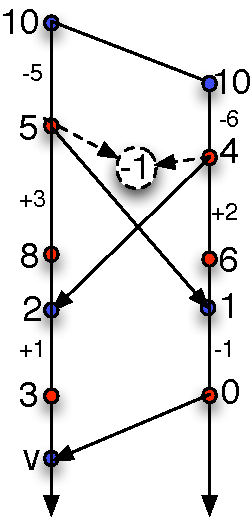
\includegraphics[scale=0.55]{Figures/2-LCAs}
}
\hfill
\subcaptionbox[] {\small
  In this example, versions $v_{13}$ and $v_{44}$ have two LCAs
  ($v_{22}$ and $v_{32}$)  despite there not being any previous merges
  between their respective branches.
  \label{fig:external-lcas}
} [0.47\columnwidth] {
  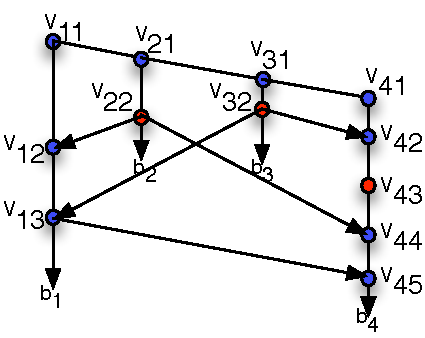
\includegraphics[scale=0.7]{Figures/2-external-LCAs}
}
\caption{Examples where merging versions have more than one LCA}
\label{fig:many-lcas}
\end{figure}

When merging two concurrent versions $v_1$ and $v_2$, the common
ancestor argument for \C{merge} must the LCA of $v_1$ and $v_2$,
without which \C{merge} may yeild unexpected results. This is
demonstrated for the grow-only counter in
Fig.~\ref{fig:merge-needs-lca}, where incorrect count is obtained if a
common ancestor that is not an LCA is used to merge 4 and 7. While in
this example there is a unique LCA for 4 and 7, in general this may
not be the case. With unrestrained branching and merging, there is no
bound on the number of LCAs a pair of versions can have.
For example, in
Fig.~\ref{fig:criss-cross-lcas}, the merge of 0 with 3 is preceded by
two ``criss-cross'' merges between their respective branches resulting
in there being two LCAs (5 and 4) for 0 and 3. Multiple LCAs can occur
even without criss-cross merges, as demonstrated by
Fig.~\ref{fig:external-lcas}. Concurrent versions with multiple LCAs
do not lend themselves to three-way merging. This problem also arises
in the context of source control systems, which employ ad hoc
mechanisms to pave way for three-way merging.  GitHub~\cite{github},
for instance, recursively merges LCAs to compute a virtual ancestor,
which then serves as the LCA for merging the concurrent versions. This
method is demonstrated for the example in
Fig.~\ref{fig:criss-cross-lcas}, where LCAs 5 and 4 of 0 and 3 are
merged (with LCA of 10) to generate -1 as the virtual LCA to merge 5
and 4. A major downside with this method is that it makes no
guarantees of the relationship between the virtual ancestor and the
concurrent versions; the former may not even be a legal ancestor of
the latter as per the semantics of the data type. For instance, the
integer type in Fig.~\ref{fig:criss-cross-lcas} may in fact represent
a bank account, which disallows any activity on the account if balance
is ever known to be less than zero. Thus, from the perspective of a
bank account, it doesn't make sense how concurrent versions 3 and 0
emerged from -1, since the only transition allowed by the semantics
from -1 is to itself. Clearly, ad hoc mechanisms, which work for the
text, may not work for more sophisticated data types.

Fortunately, unlike the source control systems where branching
structure is entirely dictated by the user, \name abstracts away the
branching structure from the programmer, hence retains the ability to
constrain it in a way that it deems fit. In particular, \name solves
the problem of multiple LCAs by suitably constraining the branching
structure such that the problem never arises. The constraints are
imposed either implicitly, as a result of how operational semantics
defines an atomic step, or explicitly, by insisting that certain
conditions be met before merging a pair of versions
(\rulelabel{E-Pull-Wait}). Firstly, the operational semantics already
disables criss-cross merges since it only ever merges versions that
are latest on their respective branches. For instance let $v_{11}$ and
$v_{21}$ be the latest versions on branches $b_1$ and $b_2$,
respectively. Meging $b_2$ into $b_1$ requires entails $v_{21}$ into
$v_{11}$ to generate version $v_{12}$ on $b_1$. Now, merging $b_1$
into $b_2$ translates to merging $v_{12}$ into $v_{21}$ (a
\emph{fast-forward} merge, in Git parlance), but not $v_{11}$ into
$v_{21}$, thus preventing a criss-cross branching structure. In other
words, a criss-cross branching structure is prevented due to the
order among merges between conflicting branches introduced as a result
of \rulelabel{E-Pull-Wait} being an atomic step. 

Secondly, we impose certain pre-conditions on the merging branches to
preempt the structure shown in Fig.~\ref{fig:external-lcas}. The
intuition is as follows: consider the branch $b_1$ at the instance of
merging $b_3$. Since it has already merged $b_2$, a version on $b_2$
($v_{22}$) could be a common ancestor for a version on $b_1$
($v_{12}$) and some other version (call it $v$). Now, if $b_1$ merges
$b_3$, same could be true of $b_3$ and $b_1$: a version on $b_3$
($v_{32}$) could be a common ancestor for the new version on $b_1$
($v_{13}$), and the other version $v$. Since $v_{22}$ is also an
ancestor of $v_{13}$, and both ancestors are not ordered by the
ancestor relation, $v_{13}$ and $v$ end up with two LCAs. In
Fig.~\ref{fig:external-lcas}, the role of $v$ is played by the version
$v_{44}$. We observe that this scenario can be prevented if, when
merging $b_3$, $b_1$ insists on an ancestor relation between the
merged version ($v_{22}$) of the $b_2$, the previously merged branch,
and the latest version of $b_3$, the current merging branch. We call
the last merged version the \emph{external locus} of the branch. By
requiring that, for every branch $b$, the external locii of $b$ at
various points in time (i.e., external locus of every prefix of $b$)
be totally ordered, we effectively enforce the invariant that for any
two common ancestors $v_1$ and $v_2$ between two versions, there
exists another common ancestor $v_3$ that succeeds $v_1$ and $v_3$ in
the ancestor relation, thereby preventing the possibility of multiple
LCAs.

%% <false>
%% Multiple versions that merge any pair of versions are totally
%% ordered. That is, if $v_1$ and $v_2$ are ancestors of $v_3$ and
%% $v_4$, then $v_3$ and $v_4$ are ordered by the ancestor relation.
%% </false>

%% If $v_1$ and $v_2$ are ancestors of $v_3$ and $v_4$, then there
%% exists a $v_5$, a successor of $v_1$ and $v_2$, and an ancestor of
%% $v_3$ and $v_4$
%% If I follow one of your locii, or you follow one of my locii, then
%% we both have same set of external common ancestors.

\begin{figure}
\centering
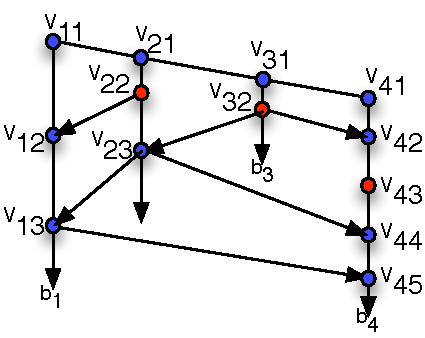
\includegraphics[scale=0.75]{Figures/legal-merge}

\caption{A legal branch history for the example in
Fig.~\ref{fig:external-lcas}}
\label{fig:legal-merge}
\end{figure}


Let us see how the aforementioned restriction allows us to merge the
branches in Fig.~\ref{fig:external-lcas} without ever creating
multiple LCAs. The legal branching history is shown in
Fig.~\ref{fig:legal-merge}. First, like in
Fig.~\ref{fig:external-lcas}, $b_2$ is merged into $b_1$ to create
$v_{12}$, and $b_3$ is merged into $b_4$ to create $v_{42}$. Thus, the
external locus of $b_1$ is $v_{22}$, and that of $b_4$ is $v_{32}$.
Observe that now $b_1$ cannot merge $b_3$, neither can $b_4$ merge
$b_2$ because $v_{22}$ and $v_{32}$ are not related by the ancestor
relation. Same applies for $b_1$ and $b_4$ because neither one's
latest version follows from other's external locus.  However, $b_2$
and $b_3$ can merge among themselves. Let us say they indeed merge to
to create a version $v_{23}$ on $b_2$. The branch $b_2$ is now
eligible to be merged into $b_1$ and also $b_4$. These merges do occur
in Fig.~\ref{fig:legal-merge} to create versions $v_{13}$ and
$v_{44}$, and making $v_{23}$ the external locus for both $b_1$ and
$b_4$. Thus, $b_1$ can now merge into $b_4$ to create version $v_{45}$
on $b_4$. Note that alternative legal histories are also possible. For
instance, $b_4$ could have skipped the merge with $v_{23}$ (hence, the
version $v_{44}$), and directly merged $v_{13}$ in the last step.
This is legal because $b_4$'s locus before the merge, $v_{32}$, is an
ancestor of the merging version $v_{13}$.

We now formalize the intuitions described above to precisely define
the notion of mergeability:

\begin{definition} [\bfseries Internal and External Ancestors]
Given a branch $b$ and a version $v\in b$, an internal ancestor of $v$
is an ancestor from the same branch $b$. An external ancestor of $v$
is an ancestor from a different branch $b'\neq b$. 
\end{definition}

\begin{definition} [\bfseries External Locus]
Given a branch $b$ and a version $v\in b$, external locus ($v_o$) of
$v$ is an external ancestor that is not an ancestor of any other
external ancestor of $v$. That is, $\under{H}{v_o \preceq v}$, and
there does not exist a $v_o' \not\in b$ such that $\under{H}{v_o'
\preceq v}$ and $\under{H}{v_o \preceq v_o'}$. 
\end{definition}

\begin{definition} [\bfseries Mergeability]
Given a history $H$, a version $v_1$ and a version $v_2$ that is not
an ancestor of $v_1$ under $H$, $v_2$ is mergeable into $v_1$ (denoted
$\under{H}{v_2 \mbleto v_1}$) iff $v_1$'s external locus is an
ancestor of $v_2$, or $v_2$'s external locus is an ancestor of $v_1$.
\end{definition}

Rule \rulelabel{E-Pull-Wait} of the reduction relation
(Fig.~\ref{fig:opsem}) is enabled only if the latest version ($v'$)
of thread $t'$'s branch is mergeable into the latest version ($v$) of
thread $t$'s branch (i.e., $\under{H}{v' \mbleto v}$). Merge computes
the latest common ancestor of $v$ and $v'$, which is 
guaranteed to be unique as per the following theorem\footnote{Proof
included in the appendix}:

\begin{theorem} [\bfseries Unique LCA]
Every pair of versions $v_1$ and $v_2$ in a legal branch history $H$ 
have a unique least common ancestor. 
\end{theorem}

The \rulelabel{E-Pull-Wait} uses the function \C{lca} to compute the
LCA of (the latest versions on) a pair of branches. The definition of
the function is standard, hence not discussed.
